
\begin{figure}[H]
\caption{PCA Reduced Embeddings with K-Means Clustering} \label{fig_clusters}
\vspace{-0.5cm}
\begin{center}
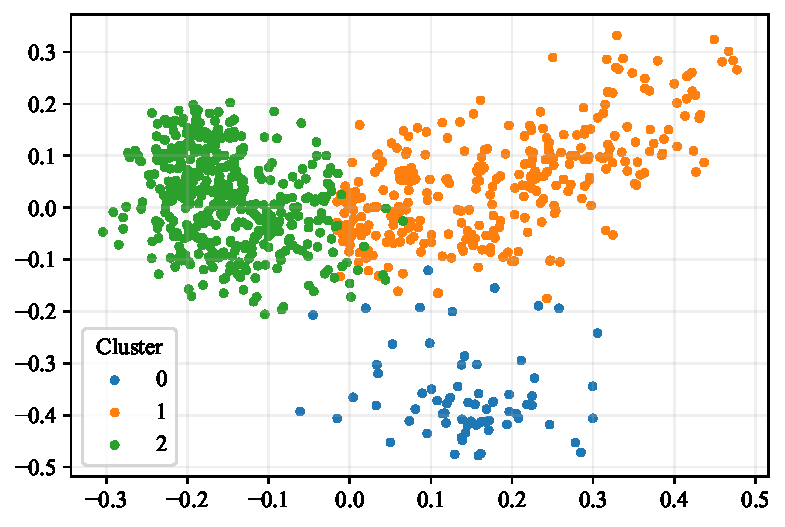
\includegraphics[width=\textwidth]{figures/fig_clusters.pdf}
\end{center}
\vspace{-0.4cm}
{\footnotesize \textit{Note}: Result of K-means clustering with three clusters on the first 10 principal components of the embedding space. The first two dimensions of the 10-dimensional subspace are shown. Each dot is an agenda item.}
\end{figure}
